\input{chapter-header.tex}
% =============================================================================
\chapter{Introduction}
\chaplabel{introduction}
\minitoc
% =============================================================================


Reflective systems are those that reason about and act upon themselves \cite{Smit84a}. A causal connection exists between the program and its representation inside the program itself as a meta-program \cite{Maes87a}. This reflective architecture introduces self-references:  an object-oriented system is composed by objects, which are instances of classes, which are also objects, and so on. These self-references, also known as meta-circularities \cite{Chib96a}, allow the manipulation of several meta-levels on one infrastructure.

Reflective systems traditionally modify their self-representation to evolve and define new abstractions. However, the self-modification approach of evolution has many drawbacks, such as making difficult the self-surgery operations~\cite{Casa09a} or the lose of the reproducibility of the system. On the other hand, non-reflective systems develop an evolution approach by recreation. Whenever a change has to be made to the system, a new system is created with the new changes applied. This approach solves many of the drawbacks of the reflective approach.

\gp{add some sentences on why it is important to evolve, which kind of software artifacts we would like to evolve, why it is challenging}

% =============================================================================
\section{The need for Software Evolution}
% =============================================================================

\gp{search for people saying the world is changing :)}
In the last years, evolving a language kernel has become an important task. Multicore hardware brought new problems on concurrency and parallelism; the \emph{cloud} increased the need for software adaptation; new resource constrained devices presenting new challenges to software developers.

% =============================================================================
\section{Resource Constrained Devices}
% =============================================================================

\gp{noury had a reference on this -> everything is going small}

%Unused deployed code units have an undesired impact when targeting a constrained infrastructure. 
%Constrained devices may present restrictive hardware such as low primary or secondary memory, or even software impositions such as the Android's Dalvik VM restriction to deploy only 65536 methods\footnote{According to dalvik's bytecode documentation~(\url{http://source.android.com/devices/tech/dalvik/dalvik-bytecode.html}), the source register accepts values between 0 and 65536.}. Big JavaScript mashup applications have an impact on loading time due to network speed and parsing time.
%These limitations may forbid the deployment of applications that contain lots of code units, or limit the amount of applications and content an user can have in its device.

%Existing solutions to this problem propose the extraction of used code units of an application to reduce their size and memory footprint. Java Micro Edition~\cite{JavaME} proposes a general purpose specialized runtime environment with no possibility of customization. Other solutions in the field propose to automatically detect and extract used code units, so called \emph{tailoring}, with static call graph construction as the most dominant technique~\cite{ShortGrov97a}. 
%Static approaches present limitations in the presence of dynamic features such as reflection or in the absence of static type annotations. Additionally, these existing solutions are generally designed to extract all used code units with no possibility for the user to customize the process of selection.

Deployed applications contain a set of code units such as classes and methods.
At run-time, required code units are loaded into RAM according to some \emph{loading strategy}.
Scripting languages such as JavaScript, Ruby, Python or PHP have an explicit loading strategy: they load and run a script file and all its declarations when an explicit import statement is found. 
Java uses a transparent code unit loading strategy based on class loaders~\cite{ShortLian98a}: a class loader loads classes on demand in a transparent way for the application code.
However, in both situations the deployed application tend to occupy more secondary memory than necessary.
Besides, an application may load a code unit that is only partially used, such as a class with some methods that are never invoked.

%Deployed object-oriented applications often contain \emph{code units}~(e.g. packages, classes, methods) that the running application never uses. 
This problem shows itself more evident and harder to control under the usage of third party software. 
Third party libraries and frameworks are designed in a generic fashion that allows multiple usages and functionalities, while applications use only few of them. 
Examples are logging libraries, web application frameworks or object-relational mappers.


%Figure~\ref{fig:unusedCodeUnits} shows a typical deployment scenario with unused code units.
%
%This problem becomes more evident with the inclusion of third party libraries~(and frameworks). 
%Third party libraries provide often a great variety of code units, usually designed in a generic fashion. 
%They allow multiple usages, while applications tend to use only some of them. 
%Additionally, application developers do not often modify and customize third party libraries to fit their needs but use them as black boxes. 
%Modifying them would mean to lose compatibility with the original development branch of the library and having deep knowledge on the library.
%
%\begin{figure}[ht]
%\begin{center}
%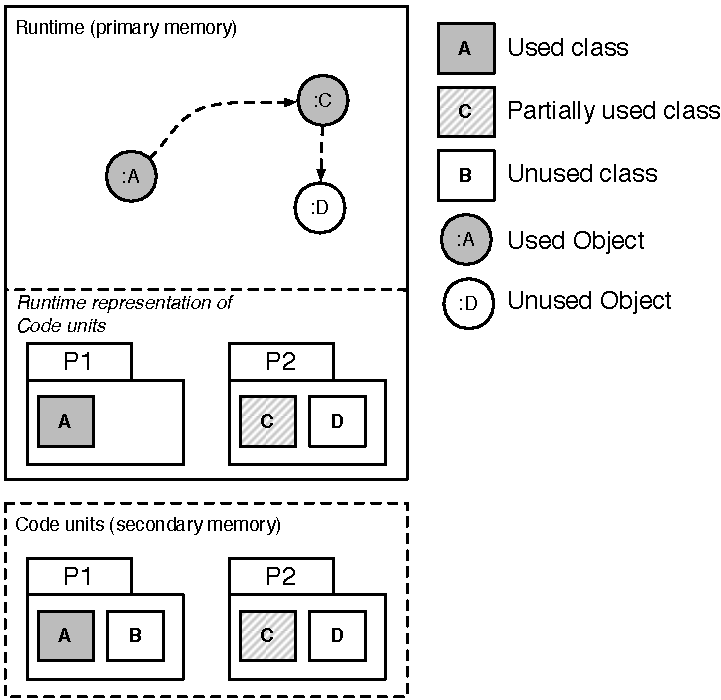
\includegraphics[width=1\linewidth]{components}
%\caption{\textbf{Unused Code Units.} Package P1 contains class A which is used during runtime and class B which is never needed and thus, not loaded. Package P2 contains class C which is partially used~(it contains methods that are never invoked) though it's completely loaded. Class D is loaded because an instance of it is created, but it is never used.\label{fig:unusedCodeUnits}}
%\end{center}
%\end{figure}

Unused code units represent serious drawbacks in constrained devices. 
First, unused code units may forbid the deployment into a constrained resource device.
It may also interfere with the deployment and usage of other applications, because of large memory footprints in both secondary~(disk storage) and primary~(RAM) memory~\cite{Mart12a} or the presence of slow networks in the case of rich web applications.
Second, some deployment targets may have an infrastructure designed in such a manner that forbids the deployment of large applications. For example, the Android's Dalvik VM restricts an application to deploy only 65536 methods.


% =============================================================================
\section{The cloud and Mobile code}
% =============================================================================

\gp{explain why code mobility is important!}

\gp{Software may adapt itself in different circumstances, which could be some times unexpected.}

Code mobility is a mechanism that allows the migration of programs between different environments. It provides support for \eg load balancing, adjusting an application's resources dynamically and functionality customization. Fuggetta et al. define informally code mobility as the capability to rebind a piece of code with the location it is running~\cite{Fugg98a}. Such rebinding may consist, depending on the style of mobility, in the mobility of execution state, application data and resources, or both of them. Execution state mobility is the ability to suspend the actual execution of a program and transfer its internal execution information~(\eg code, execution stacks, instruction pointers) to some other environment. Data mobility is the ability to transfer the application's data~(\eg objects, database connections, files) between different environments.

Application data is usually composed by elements of different nature. Files are used for configuration and logging. Network connections such as sockets are used to communicate with remote systems. External libraries provide with code reuse. We can also find objects local to the application, of two different categories: domain objects modeling the application's specific concerns and application objects modeling those concerns that are cross-cutting between applications.

In our experience manipulating the language kernel of Pharo, we identified several cases where data mobility presents some issues. We can generalize those issues as mobility either \emph{in time}~(\ie creating or recreating a program), or \emph{in space}~(\ie moving a program between different environments):

\begin{description}
\item[Transporting code in space.] When moving a program from one environment to another one, some of its state becomes invalid. For example, files existing in one machine will not exist in some other. Because of this, the migration mechanism should be aware of the state it migrates, to either reinitialize it, re-bind it in the new environment, or by keep it with its same value~\cite{Unga95a}.

\item[Transporting code in time.] Image-based systems allow one to persist the state of a program to restart it at some other point of time from the last check-point, introducing the idea of \emph{program sessions}: every time the system is restarted, a new \emph{session} is started. These programming sessions introduce the concern of \emph{session specific state} \ie state that is only valid during a programming session. The mechanism in charge of stopping and restarting the image has to recognize the session specific state to re-initialize or rebind it every time a new session is started.

\end{description}

% =============================================================================
\section{Multicore Architectures}
% =============================================================================

\gp{maybe we don't have to include this... since we do nothing with multicore, it's just bluffing... If it goes somewhere, it should go to future work?}

% =============================================================================
\section{What to Evolve?}
% =============================================================================

Modern object-oriented programming languages possess a \emph{runtime system} that implements a set of services~(\eg memory manager, a (byte)code interpreter and a process/thread manager) and an execution model for running programs~(\eg an object format, a class or prototype model). Programming languages should conform to the execution model provided by the runtime system to run on it. Programming languages such as Java, Python, JavaScript and Prolog encapsulate their runtime systems inside a virtual machine~(VM).

Simplistically, running a program written in any of these languages consists in launching the respective VM and give it the desired program as input. Launching the VM initializes its internal structures~(\ie allocates the heap, initializes threads and input/output streams, loads external libraries, etc.) and \textbf{the language kernel}. The language kernel is the set of objects and functions/methods\footnote{these constructions vary from language to language.} available to a program from the very beginning. It includes basic objects such as booleans, numbers and strings as well as basic language libraries\gp{give a better example}.

Amongst programming languages we identify reflective languages as those that can reason about and act upon themselves. Reflection works thanks to a self-describing architecture, so called \emph{reflective architecture}~\cite{Smit84a}. We find reflective architectures in languages such as \eg Lisp, Ruby and Python. These reflective architectures are based on the notion of causal connection between the system and its meta-level~\cite{Maes87a}. A causal connection is a link between two elements in a system such that if any of those element changes, the others will be impacted by that change. For example, in Ruby and Smalltalk, a class is an object and changing it will affect all its instances. Thus, reflective architectures impact on the language kernels built on top of them: reflective language kernels are considered to be defined by themselves, including circular definitions that should be consistently initialized and maintained.

\subsection{Virtual Machines}

\subsection{Language Kernels}

\subsection{Application Software}

% =============================================================================
\section{On Evolution Methodologies}
% =============================================================================

\subsection{Recreation: The case of non-reflective languages}

Non-reflective software evolve by recreation. This means they evolve by generating from scratch of a new version of it. These systems are generated by a system \emph{builder} which takes a \emph{specification} of the system and builds the new system (\autoref{fig:generate_system}).
The specification of the system must include the elements and behavior of the new system. Sometimes it can also include some order in which the system should be built.
For example, to recreate a C program, a C compiler (the system builder) will take the source code of the program (the specification) as input.

\begin{figure}[!ht]
\begin{center}
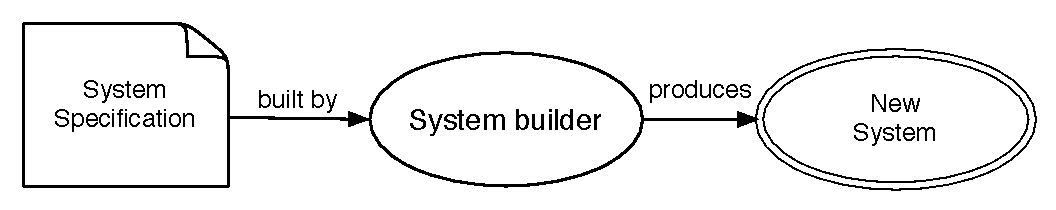
\includegraphics[width=0.6\linewidth]{system_recreation}
\caption{Process to generate a new system.\label{fig:generate_system}}
\end{center}
\end{figure}

\autoref{fig:evolution_recreation_systems} depicts how a system such as a C compiler can evolve using this approach.
At the first stage, the compiler and its source code represent version 1 of the system.
A change is introduced in the source code of the compiler, to depict version 2 of the source code.
The version 1 of the compiler, which conforms to the version 1 of the source code, is now \emph{out of synchronization} with the new source code or specification.
The source code version 2 is used to generate the compiler version 2.
Finally, the compiler version 2 conforms to the source code in version 2.

%\begin{figure}[!ht]
%\begin{center}
%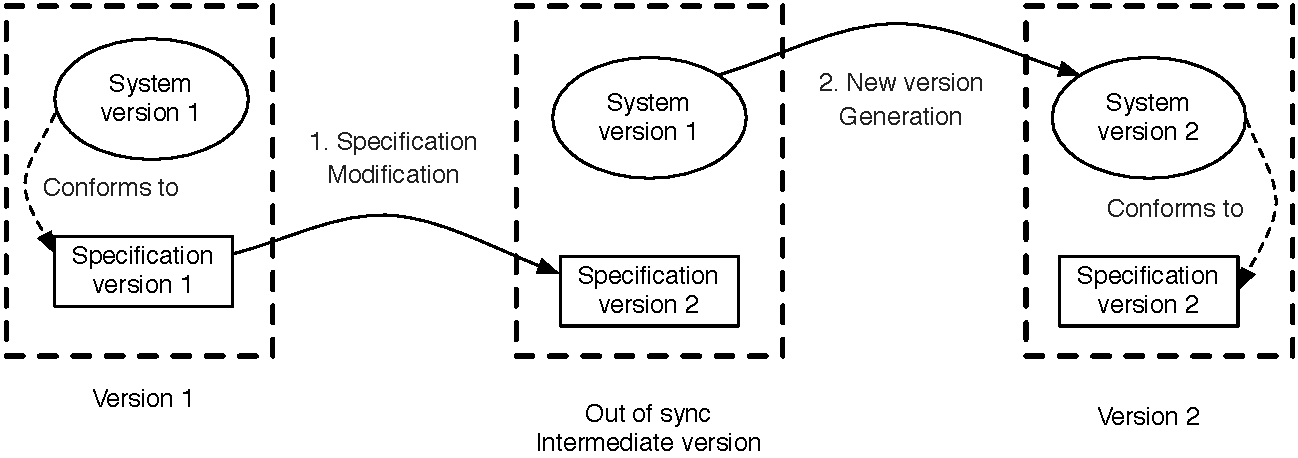
\includegraphics[width=0.5\linewidth]{evolution_recreation_systems2}
%\caption{Evolution of a non causally connected system by recreation after each modification of the system specification\label{fig:evolution_recreation_systems}}
%\end{center}
%\end{figure}

This approach provides a deterministic and explicit process to build a new version of the system from scratch.
Multiple changes can be applied to the specification while it is out of synchronization with the system.
These changes will be applied atomically in the new system when it is generated.
On the other hand, the main drawback of this approach is the slow feedback loop in the development process.
The specification and the system can stay out of synchronization during a large period of time without providing information about errors and mistakes.
Thus, it is easier to reach non-working stages.

%A particular case of system recreation is the introduction of the newly generated system into the generation process. The newly generated system can be used as a system builder in the process of generating a new system. This case, commonly known by its usage in compilers, is normally referred as \emph{bootstrapping}.


\subsection{Self-Modification: The case of reflective languages}

\gp{emphasize this is the way for 0-down systems, since we cannot stop them to update/change them}

Reflective systems are those that reason about and act upon themselves~\cite{Smit84a}.
They embed their structure and behavior in themselves in a causally connected way.
Causal connections enable a reflective system to modify itself and reflect their changes immediately.
The ability to change itself is called \emph{self-modification}.

A system evolves by self-modification when it applies \emph{deltas} directly on itself to alter its representation. 
A delta is an atomic and indivisible change of the system, such as the introduction of a class or a method, or the assignment of a variable.
Each delta applied to the system triggers a migration of the entities in the system, which automatically reflect the change.
For example, adding an instance variable into a class definition migrates all its instances by adding them the new extra slot.
Thus, the system is at any moment during its life synchronized with its internal representation.\gp{say it is a causal connection}
To evolve a system to a desired state, a \emph{stream} of deltas in a specific order must be applied to it.
\autoref{fig:evolution_reflective_systems} shows how a stream of changes \{$\Delta_1, \Delta_2$\} is applied to version 1 of a reflective system to obtain, in order, version 2 and version 3.

\begin{figure}[!ht]
\begin{center}
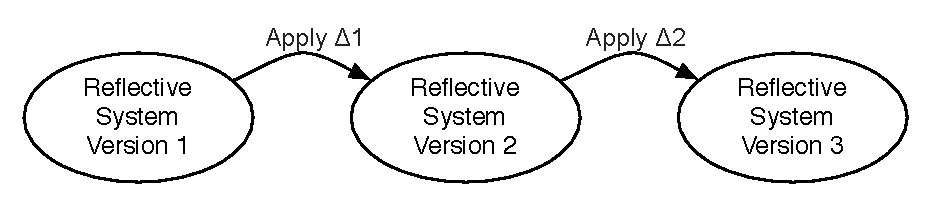
\includegraphics[width=0.6\linewidth]{evolution_reflective_systems}
\caption{Evolution of a reflective system by self-modification\label{fig:evolution_reflective_systems}}
\end{center}
\end{figure}

%Pharo~\cite{Blac09a} and Squeak~\cite{Blac07a} are object-oriented systems evolving traditionally by self-modification. These systems store their state and all their objects in an \emph{image}. A snapshot of the image can be stored at any time, creating a \emph{backup} of the state of the system. When the image is restarted, its state is the same as it was at the last snapshot. These systems evolve by applying deltas on themselves and making a snapshot of the new state of the system.

%Some tools such as the SystemTracer in Squeak~\cite{Blac07a} can produce a new image by applying certain transformations (like pointer representation modification) to the objects.

\gp{review from here}
Based on our experience maintaining and evolving them during several years \cite{Denk07a}, we list some problems appearing in these evolutive approach: 
\begin{description}

\item[\emph{Evolving requires sequences of side effects.}] A stream of ordered and compatible delta have to be applied to the system to reach a particular version of it. A delta could depend on the deltas applied before it, and enable the application of its subsequent ones. It may be difficult to order the deltas of big changes to get the system to a specific state. 
Consider for example a Smalltalk system with an \ct{Array} class defining an iterator method \ct{do:}.
This iterator method is used in critical parts of the system.
A refactor to move the iteration method to the superclass of the Array class consists basically in the removal of the method from the \ct{Array} class and the introduction into its superclass.
However, removing first the method from the \ct{Array} class leads to an irrecoverable system crash.
To perform this refactor safely, the order in which the actions are realized must be reverted: first the iterator method must be introduced into the superclass.
So, when removing the method in the Array class, the method is looked up correctly.
Evolution by self-modification lacks a way to apply several changes atomically to a system.

\item[\em{Impossibility to recover from system crashes.}] When doing self brain surgery~\cite{Casa09a} in the system (modifying parts of the system that are used to performing the changes themselves), a delta in a given stream may leave the system in a broken state. This leads to the lose of the already applied deltas. The system relies on its backups or snapshots to recover to a previous state, making difficult and tedious the process to evolve the system to versions involving many critical deltas. 

\item[\emph{Unmaintained code.}] The initialization methods of certain classes are not systematically exercised. This makes the code of these initializations get easily broken or obsolete. For example, the character table in the system can be modified by altering it directly without updating its initialization code. Additionally, methods can refer to inexistent classes or send messages that are not understood any more. Such a situation presents a problem when these parts of the system have to be re-initialized again.

\item[\emph{Lack of support for building up the system.}] The system is represented by a monolithic image containing lots of packages not needed for every usage, such as the UI, networking, debugger or compiler. This monolithic image, due to its size, represents a problem when deploying it on a resource constrained environment such as embedded devices. Building a system with only the necessary parts is nowadays only feasible by image shrinking with self-modification, making the system unstable during its modification.
The image has been a big monolithic unit since years, leading to hidden and hard to break dependencies in it, making the shrinking process tedious. Additionally, the dynamic nature of the system and the use of reflective features breaks static analysis when trying to understand the hidden dependencies \cite{Livs05a}.
\end{description}


% =============================================================================
\section{Problem Statement}
% =============================================================================

\gp{write from scratch}
Following the problem description listed in the above introduction we identified the following abstract concerns with existing reflective languages and their \VMs.
%
\begin{itemize}
	\item Reflection and in special behavioral reflection comes at a significant cost due to reification overhead.
		
	\item Intercession is limited to language-side.
	\VMs are not accessible from language-side and they are usually have no reflective properties at runtime. 
	
	\item Existing approaches to a unified model between the \VM and the language-side are holistic, there is no intermediate solution available.
\end{itemize}

\noindent Out of these general problems concerning reflection in high-level languages we see that they have a low-level root.
To address the unification of the language-side and \VM-side we have to grant more access to the language-side.
This includes interacting directly with low-level native instructions.
A similar problem has been solved by applying high-level low-level programming in a more static environment \cite{Fram09a,Graal}.
The approach outlined by Frampton et al. uses a high-level framework to generate native code at compile-time.
We see that their approach has not yet been applied in a more dynamic environment where native code has to be generated at runtime.
Hence we focus on the following concrete problems we wish to solve in this thesis.

\begin{description}
	\item[Problem 1:] High-level low-level programming is not available at runtime and from language-side.
	
	\item[Problem 2:] Intercession is limited to language-side.
	\VMs are not accessible from language-side and they are usually have no reflective properties at runtime.
	
	\item[Problem 3:] High-level low-level programming has not yet been provided as an incremental extension to an existing language runtime.
\end{description}

% =============================================================================
\section{Thesis Outline}
% =============================================================================
%\sm{This dissertation structure is different to what I am used to. At least the way you announce the purpose of the chapters is not what I would expect.
%In my diss, everything revolves around one thesis, here, it is a number of things listed one after another, don't see the central motive I would expect}

\gp{write from scratch, left for the end}
\begin{description}
\item[\chapref{background}] sheds light on the context of this work.
	We present a quick overview of language-side reflection followed by a development of \VM-level reflection.
	We find that mostly metacircular \VMs provide limited \VM-level reflection and thus we present several high-level language \VMs falling into this category.
	We conclude that there is only two research \VM that has a uniform model for \VM and language-side.
	Among them is \P a research \ST \VM we contributed to previous to working on this dissertation.

%\item[\chapref{reification}] focuses on language-side applications that simplify the interaction with the underlying \VM.
%	We present a custom inspector framework that is now used by default in \PH.
%	As a second part we explain how we introduced first-class layouts and slots to \PH to reify the low-level structural layout of objects.
%	Both projects are crucial for metacircular \VM development and are direct results from the research conducted on the \P \VM.

\item[\chapref{benzo}] describes a high-level low-level programming framework named \B.
	The core functionality of \B is to dynamically execute native-code generated at language-side.
	\B allows us to hoist typical \VM plugins to the language-side.
	Furthermore we show how code caching makes \B efficient and users essentially only pay a one-time overhead for generating the native code.
	
\item[\chapref{ffi}] presents \NB, a stable foreign function interface (\FFI) implementation that is entirely written at language-side using \B.
	\NB is a real-world validation of \B as it combines both language-side flexibility with \VM-level performance.
	We show in detail how \NB outperforms other existing \FFI solutions on \PH.

\item[\chapref{validation}] focuses on two further \B applications.
	In the first part we present \WF a framework for dynamically generating primitives at runtime.
	\WF extends the concept of metacircularity to the running language by reusing the same sources for dynamic primitives that were previously used to generate the static \VM artifact.
	In a first validation we show how \WF outperforms other reflective language-side solutions to instrument primitives.
	
	In a second part of \chapref{validation} we present \NBJ a prototype \JIT compiler that is based on \B.
	\NBJ shows the limitations of the \B approach as it required a customized \VM to communicate with the existing \JIT interface for native code.
	Our prototype implementation generates the same native code as the existing \VM-level \JIT, however, it is currently limited to simple expressions.
	\NBJ shows that for certain applications a well-define interface with the low-level components of the \VM is required.

\item[\chapref{future}] summarizes the limitations of \B and its application.
Furthermore we list undergoing efforts on the \B infrastructure and future work.

\item[\chapref{conclusion}] concludes the dissertation.

\end{description}

% =============================================================================
\input{chapter-footer.tex}
% =============================================================================